\documentclass{standalone}
\usepackage{tikz}
\usepackage{amsmath}

\begin{document}

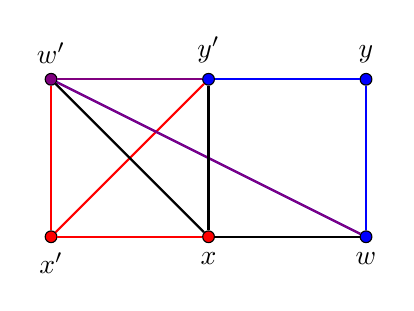
\begin{tikzpicture}

% Define colors
\definecolor{red}{rgb}{1,0,0}
\definecolor{blue}{rgb}{0,0,1}
\definecolor{violet}{rgb}{0.5,0,0.5}

% Nodes
\node[draw, circle, fill=red, inner sep=1.5pt, label=below:$x'$] (x') at (0,0) {};
\node[draw, circle, fill=red, inner sep=1.5pt, label=below:$x$] (x) at (2,0) {};
\node[draw, circle, fill=blue, inner sep=1.5pt, label=below:$w$] (w) at (4,0) {};
\node[draw, circle, fill=violet, inner sep=1.5pt, label=above:$w'$] (w') at (0,2) {};
\node[draw, circle, fill=blue, inner sep=1.5pt, label=above:$y'$] (y') at (2,2) {};
\node[draw, circle, fill=blue, inner sep=1.5pt, label=above:$y$] (y) at (4,2) {};

% Edges
\draw[red, thick] (x') -- (x);
\draw[red, thick] (x') -- (w');
\draw[red, thick] (x') -- (y');
\draw[blue, thick] (y') -- (y);
\draw[blue, thick] (w) -- (y);
\draw[blue, thick] (w) -- (w');
\draw[violet, thick] (w') -- (y');
\draw[violet, thick] (w') -- (w);
\draw[black, thick] (x) -- (w);
\draw[black, thick] (x) -- (y');
\draw[black, thick] (x) -- (w');

\end{tikzpicture}

\end{document}